%第3章


\section{商品識別システムの概要}

商品識別システムでは,WebカメラとRaspberry Pi,各種センサを各買い物カゴに設置し,従来のセルフレジやセミセルフレジに比べて安価かつ簡単に決済できる買い物を提案する.

本研究において対象として設定したスーパーマーケットを下記の表\ref{taisho}に示す.


\begin{table}[htb]
\begin{center}
\caption{対象スーパーマーケット}
\begin{tabular}{|l|c|c|c|} \hline
店舗 & 売場面積(平方メートル) & レジ台数 & カゴ数 \\ \hline
小規模店舗,中規模店舗 & 1,200 & 7台 & 90個 \\ \hline
\end{tabular}
\label{taisho}
\end{center}
\end{table}


表\ref{taisho}を対象として設定した理由を下記に述べる.本研究では小規模店舗と中規模店舗のスーパーマーケットを対象とする.小規模店舗は「売場面積$800m^2未満」あるいは「売場面積800m^2~1,200m^2未満」の店舗,中規模店舗は「売場面積800m^2~1,200m^2未満」または「売場面積1,200m^2~1,600m^2未満」の店舗を指す\cite{super}.本研究では,小規模店舗と中規模店舗の平均である,売り場面積1,200m^2の店舗を本研究の対象の店舗とする.売場面積1,000m^2あたりレジ台数は,平均5.7台のため,対象の売場面積1,200m^2の店舗ではレジ台数平均6.84台と仮定できる\cite{super}.四捨五入してレジ台数は7台とし,対象のレジ台数とする.また,売場面積が1,200m^2~1,600m^2$のスーパーマーケットの場合,平日レジ一台あたり一日客数は中央値として225.5人である\cite{super}.なお,平均営業時間は12.3時間のため,一時間あたり約18人の客がレジを使用すると予測できる\cite{super}.1人につき1個のカゴを使用しピーク時等の客入りを5倍,かつ店内に滞在する時間を1人につき1時間と仮定すると,約90個のカゴが必要と仮定した.


本システムを使用する流れを図\ref{summary1}に示す.


\begin{figure}[htbp]
\centering
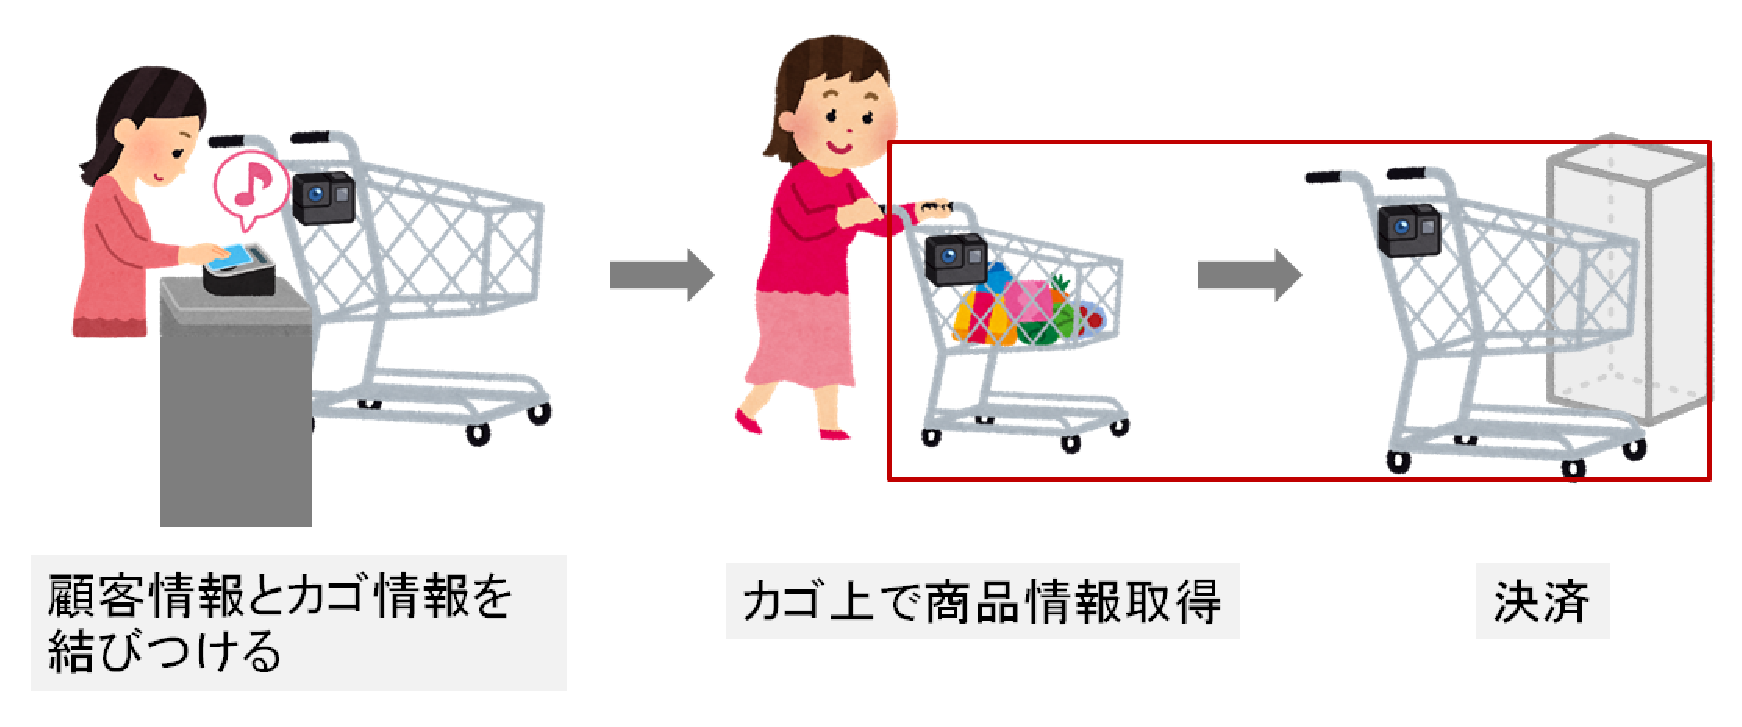
\includegraphics[width = 15cm]{./picture/summary1.eps}
\caption{商品識別システム全体の流れ}
\label{summary1}
\end{figure}



まず,顧客情報をカゴ情報と結び付ける.その後顧客はカゴに通常通り商品を入れる.その際,センシング技術を用い,カゴ上で商品情報を取得しサーバへ情報を送信する.買い物を終える際は,カゴを返却するだけで決済が行われる流れとなる.本研究では商品識別システム全体の流れについて設計を行ったが,最終的には,優先度が高い機能とした図\ref{summary1}にある赤枠の範囲である,カゴ上で商品情報を取得し決済を行う部分を開発対象とした.上記範囲の商品識別システムのイメージ図を以下の図\ref{summary2}に示す.


\begin{figure}[htbp]
\centering
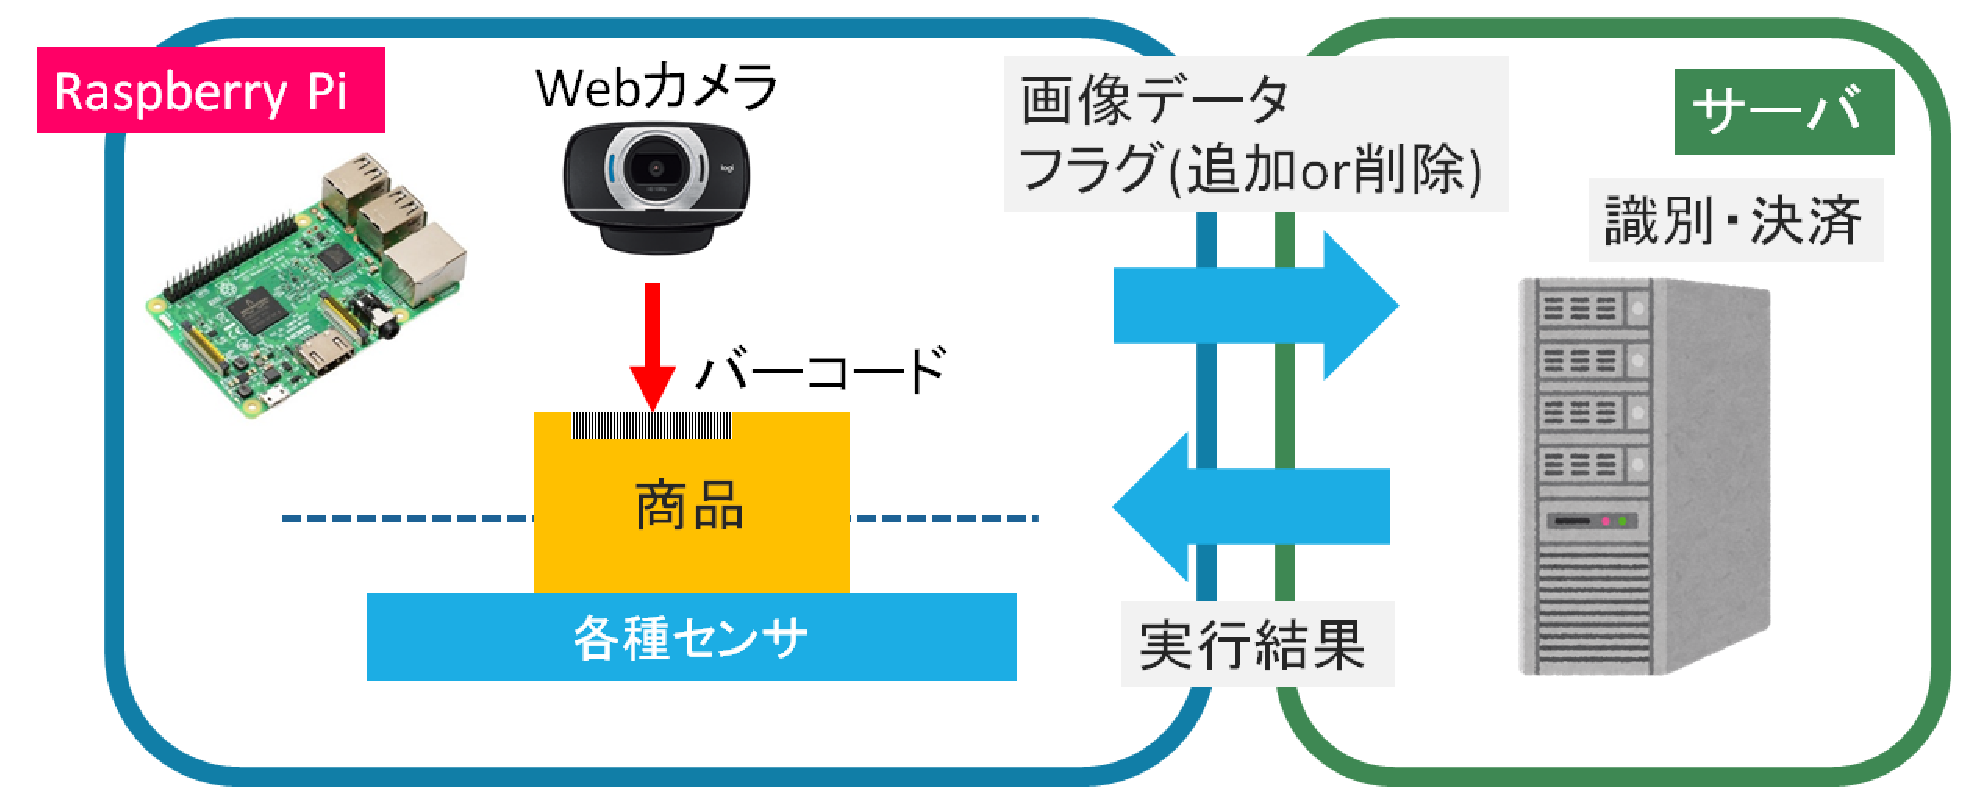
\includegraphics[width = 15cm]{./picture/summary2.eps}
\caption{商品識別システムのイメージ図}
\label{summary2}
\end{figure}


商品識別システムは識別・決済等を行うサーバ側,Raspberry PiとWebカメラ,各種センサを設置した買い物カゴであるエッジ側の2つのパートで構成される.商品を各種センサが検知した際,Webカメラで商品のバーコードを撮影し,画像データ等をサーバへ送信する.サーバでは商品のバーコード情報等を識別し,カゴに入れた商品の種類,金額,賞味期限,入れる時間などの情報を決済システムに一時的に保存し,仮登録する.ユーザはショッピングが終了する時点(決済ゲージを通る)に仮登録した商品の最終決済を行う.システムの実装は,サーバ側を段原丞治が,エッジ側を真鍋樹が担当した.本論文ではシステム全体の流れを商品識別システムと呼び,システム全体の中でのモビリティショッピング端末の開発を筆者が担当した.